\documentclass[12pt,a4paper,openany]{book}
\usepackage{amssymb}
\usepackage{fontspec}
\usepackage{amsmath}
\usepackage{amsfonts}
\usepackage[mathscr]{eucal}
%\usepackage{accents}
%\usepackage{statex}
\usepackage{graphicx}

\setromanfont{SimSun}
\setmainfont{SimSun}

\XeTeXlinebreaklocale "zh"
\XeTeXlinebreakskip = 0pt plus 1pt

\newtheorem{example}{例} 
\newtheorem{theorem}{定理}[section]
\newtheorem{definition}{定义}[section]
\newtheorem{axiom}{公理}[section]
\newtheorem{property}{性质}[section]
\newtheorem{proposition}{命题}[section]
\newtheorem{lemma}{引理}[section]
\newtheorem{corollary}{推论}[section]
\newtheorem{remark}{注解}
\newtheorem{condition}{条件}
\newtheorem{conclusion}{结论}
\newtheorem{assumption}{假设}
\newtheorem{exercise}{解答}[chapter]
\newtheorem{answer}{解答}[chapter]

\newcommand\relphantom[1]{\mathrel{\phantom{#1}}}
\newcommand\num[1]{\left\Vert{#1}\right\Vert}
\newcommand\Hom{\text{Hom\,}}
\newcommand\Tr{\text{Tr\,}}
\newcommand\Ker{\text{Ker\,}}
\newcommand\Image{\text{Im\,}}
\newcommand\rank{\text{rank\,}}
\newcommand\tr{\text{tr\,}}

\DeclareMathOperator{\esssup}{ess\,sup}

\makeatletter
\def\wideubar{\underaccent{{\cc@style\underline{\mskip10mu}}}}
\def\Wideubar{\underaccent{{\cc@style\underline{\mskip8mu}}}}
\def\diam{\text{diam}}
\makeatother

\makeatletter
\def\widebar{\accentset{{\cc@style\underline{\mskip10mu}}}}
\def\Widebar{\accentset{{\cc@style\underline{\mskip8mu}}}}
\makeatother


\title{深度学习}
\author{虞朝阳}

\begin{document}

\frontmatter
\frontmatter
\begin{titlepage}
\maketitle
\end{titlepage}
\setcounter{page}{0}
\chapter{前言}
这是看深度学习方面的书或者资料摘录的东西,有些内容来自网络,有些内容来自书本。

\tableofcontents

\mainmatter
\chapter{一些基本内容}
\section{欠拟合和过拟合}
欠拟合的模型对于已有数据的匹配性很差,过拟合的模型能很好匹配训练数据,但是对于测试数据或者说新数据的匹配性很差。

在解决欠拟合问题时,主要从以下三方面入手。(1)增加特征项;(2)构造复杂的多项式;(3)减少正则化参数。

在解决过拟合问题时,主要从以下三方面入手。(1)增大训练的数据量;(2)采用正则化方法;(3)Dropout方法。

\section{损失函数}
常用的损失函数有均方误差函数,均方根误差函数,平均绝对误差函数。分别是下面三个:
\[
\begin{aligned}
MSE &= \frac{1}{N}\sum_{i=1}^{N}{(y_{true}^i - y_{pred}^i)^2} \\
RMSE &= \sqrt{\frac{1}{N}\sum_{i=1}^{N}{(y_{true}^i - y_{pred}^i)^2}} \\
MAE &= \frac{1}{N}\sum_{i=1}^{N}{|(y_{true}^i - y_{pred}^i)|}
\end{aligned}
\]


\section{优化函数}
目前使用的方法基本是梯度下降法,最常使用的是一阶优化函数。所谓梯度是多元函数的各个偏导数形成的向量。例如二元函数$f(x,y)$的梯度就是$(\frac{\partial{f}}{\partial{x}}, \frac{\partial{f}}{\partial{y}})$。梯度下降(GD)的基本原则是按照如下方式更改参数:
\[
\theta_j = \theta_j - \eta \times \frac{\partial{J(\theta_j)}}{\partial{\theta_j}}
\]
一些常见的变形有批量梯度下降(BGD),随机梯度下降(SGD),Adma。

\section{激活函数}
激活函数提供了非线性,从而提高了神经网络应对复杂问题的能力。常见的几个激活函数有Sigmoid函数,tanh函数,ReLU函数。

(1)Sigmoid函数
\[
f(x) = \frac{1}{1 + e^{-x}}.
\]

(2)tanh函数
\[
f(x) = \frac{e^x - e^{-x}}{e^x + e^{-x}}.
\]

(3)ReLU函数
\[
f(x) = \max(0, f(x)).
\]

\section{卷积神经网络(CNN)}
卷积神经网络中有几个经常出现的概念:卷积层(Convolution Layer),池化层(Pooling Layer),全连接层。

卷积层的主要作用是对输入的数据进行特征提取,完成该功能的是卷积层中的卷积核。这一层有几个主要输入参数:卷积核的大小,移动步长,元素填充方式(使用填充的像素层数表示)。输出参数是卷积核参数。下面公式用于计算输入图像经过一轮卷积操作之后输出图像的宽度和高度:
\[
\begin{aligned}
W_{output} &= \frac{W_{input} - W_{filter} + 2P}{S} + 1 \\
H_{output} &= \frac{H_{input} - H_{filter} + 2P}{S} + 1
\end{aligned}
\]
这里filter下标的就是卷积核的参数,S表示卷积核的步长,P表示边缘像素填充层数。

池化层可以被看作提取数据核心特征的方式,可以实现对原始数据的压缩,大量减少参与模型计算的参数。最常被用到的是平均池化层和最大池化层。池化层的主要输入参数是滑动窗口的高度和宽度,步长。下面公式用于计算输入图像经过一轮池化操作之后输出图像的宽度和高度:
\[
\begin{aligned}
W_{output} &= \frac{W_{input} - W_{filter}}{S} + 1 \\
H_{output} &= \frac{H_{input} - H_{filter}}{S} + 1
\end{aligned}
\]

全连接层的作用是将输入图像在经过卷积和池化操作后提取的特征进行压缩,并且根据压缩的特征完成模型的分类。

\section{AlexNet模型}
LeNet模型是由LeCun在1989年提出的历史上第一个真正意义上的卷积神经网络模型。目前最常被使用的是1998年出现的改进版本LeNet-5。Hinton课题组为了证明深度学习的潜力,在2012年的ILSVRC(ImageNet Large Scale Visual Recognition Competition)比赛中使用了AlexNet搭建了卷积神经网络模型,并通过该模型在这次比赛中一举夺得冠军。

\begin{figure}[h]%%图	
\centering  %插入的图片居中表示	
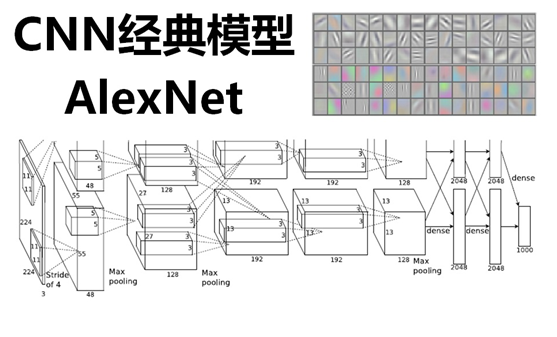
\includegraphics[width=0.7\linewidth]{figures/AlexNet.png}  %插入的图,包括JPG,PNG,PDF,EPS等,放在源文件目录下	
\caption{AlexNet模型}  %图片的名称	
\label{fig:AlexNet}   %标签,用作引用
\end{figure}

AlexNet模型包含了INPUT层、Conv1层、MaxPool1层、Conv2层、MaxPool2层、Conv3层、Conv4层、Conv5层、MaxPool3层、FC6层、FC7层、FC8层和OUTPUT层。

(1)INPUT层:输入层,默认的输入数据是维度为$224 \times 224 \times 3$的图像,也就是图像的高度和宽度均为224,色彩通道为RGB三个通道。

(2)Conv1层:使用的卷积核滑动窗口为$11 \times 11 \times 3$,步长为4,Padding为2,可以得到输出的特征图的高度和宽度为$55 = \frac{224 - 11 + 4}{4} + 1$,同时这个卷积层要求最后输出深度为96的特征图,所以需要96次卷积。最后得到输出的特征图的维度为$55 \times 55 \times 96$。按照我的理解,这里的96可以人为设定,例如VGG选择的是64。

(3)MaxPool1层:最大池化层,滑动窗口为$3 \times 3 \times 96$,步长为2,池化操作得到的输出特征图的高度和宽度为$27 = \frac{55 - 3}{2} + 1$,最后得到的输出的特征图的维度为$27 \times 27 \times 96$。

(4)Conv2层:使用的卷积核滑动窗口为$5 \times 5 \times 96$,步长为1,Padding为2,可以得到输出的特征图的高度和宽度为$27 = \frac{27 - 5 + 4}{1} + 1$,最后得到输出的特征图的维度为$27 \times 27 \times 256$。256是这个卷积层要求的。

(5)MaxPool2层:最大池化层,滑动窗口为$3 \times 3 \times 256$,步长为2,池化操作得到的输出特征图的高度和宽度为$13 = \frac{27 - 3}{2} + 1$,最后得到的输出的特征图的维度为$13 \times 13 \times 256$。

(6)Conv3层:使用的卷积核滑动窗口为$3 \times 3 \times 256$,步长为1,Padding为1,可以得到输出的特征图的高度和宽度为$13 = \frac{13 - 3 + 1}{1} + 1$,最后得到输出的特征图的维度为$13 \times 13 \times 384$。384是这个卷积层要求的。

(7)Conv4层:使用的卷积核滑动窗口为$3 \times 3 \times 384$,步长为1,Padding为1,可以得到输出的特征图的高度和宽度为$13 = \frac{13 - 3 + 2}{1} + 1$,最后得到输出的特征图的维度为$13 \times 13 \times 384$。384是这个卷积层要求的。

(8)Conv5层:使用的卷积核滑动窗口为$3 \times 3 \times 384$,步长为1,Padding为1,可以得到输出的特征图的高度和宽度为$13 = \frac{13 - 3 + 2}{1} + 1$,最后得到输出的特征图的维度为$13 \times 13 \times 256$。256是这个卷积层要求的。

(9)MaxPool3层:最大池化层,滑动窗口为$3 \times 3 \times 256$,步长为2,池化操作得到的输出特征图的高度和宽度为$6 = \frac{13 - 3}{2} + 1$,最后得到的输出的特征图的维度为$6 \times 6 \times 256$。

(10)FC6层:输入的特征图的维度为$6 \times 6 \times 256$,首先需要对输入的特征图进行扁平化处理,将其变成维度为$1 \times 9216$的输入特征图。本层要求输出数据的维度是$1 \times 4096$,需要一个维度为$9216 \times 4096$的矩阵完成输入数据和输出数据的全连接,最后得到输出数据的维度为$1 \times 4096$。

(11)FC7层:输入的特征图的维度为$1 \times 4096$,本层要求输出数据的维度是$1 \times 4096$,需要一个维度为$4096 \times 4096$的矩阵完成输入数据和输出数据的全连接,最后得到输出数据的维度为$1 \times 4096$。

(12)FC8层:输入的特征图的维度为$1 \times 4096$,本层要求输出数据的维度是$1 \times 1000$,需要一个维度为$4096 \times 1000$的矩阵完成输入数据和输出数据的全连接,最后得到输出数据的维度为$1 \times 1000$。

(13)OUTPUT层:输出层最后得到输入图像对应1000个类别的可能性值。将全连接层最后输出的维度为$1 \times 1000$的数据传递到Softmax激活函数中,就得到1000个全新的输出值,也就是模型预测的输入图像对应1000个类别的可能性值。




\end{document}
